% ============================================================================
% CHAPITRE 7 — SPRINT 4 : INTÉGRATION ET DÉPLOIEMENT
% ============================================================================

\section{Introduction}

Ce chapitre présente le quatrième et dernier sprint du projet Guidni, consacré à l'intégration
des deux sous-systèmes (agent planificateur et moteur de recommandation), au déploiement en
environnement de production, et à la démonstration finale de la plateforme complète. Le sprint
couvre également la mise en place des endpoints de santé, du tableau de bord administrateur,
et de la documentation technique.

Le sprint 4 clôture le cycle de développement Scrum en livrant un produit potentiellement
livrable qui combine toutes les fonctionnalités développées dans les sprints précédents.


% ────────────────────────────────────────────────────────────────
\section{Sprint 4 Planning}
% ────────────────────────────────────────────────────────────────

\subsection{Objectif du Sprint 4}

L'objectif du Sprint 4 est triple~:
\begin{enumerate}
    \item \textbf{Intégrer} les deux sous-systèmes développés séparément (planificateur et
          recommandation) dans une codebase unifiée sans conflits de base de données.
    \item \textbf{Déployer} le système sur un serveur de production avec monitoring, logs et
          endpoints de santé opérationnels.
    \item \textbf{Démontrer} la plateforme complète via un scénario utilisateur réaliste couvrant
          l'ensemble des fonctionnalités.
\end{enumerate}

\subsection{Sprint Backlog du Sprint 4}

Le tableau~\ref{tab:sprint4_backlog} liste les user stories sélectionnées pour ce sprint avec
leur estimation T-Shirt et leur statut de completion.

\begin{table}[H]
    \centering
    \caption{Sprint Backlog — Sprint 4}
    \label{tab:sprint4_backlog}
    \small
    \begin{tabular}{p{1cm} p{6cm} p{2cm} p{2cm} p{3cm}}
        \toprule
        \textbf{ID} & \textbf{User Story} & \textbf{Taille} & \textbf{Statut} & \textbf{Livrable} \\
        \midrule
        US-4.1 & Intégrer les tables planificateur + recommandation & M & Done & Schéma DB unifié \\
        US-4.2 & Implémenter endpoint GET /health & S & Done & Health check opérationnel \\
        US-4.3 & Créer dashboard admin rebuild-index & M & Done & Endpoint POST /admin/rebuild-index \\
        US-4.4 & Documenter l'API OpenAPI & S & Done & Swagger UI à /docs \\
        US-4.5 & Configurer logging rotatif & S & Done & Logs info/debug séparés \\
        US-4.6 & Tester scénario E2E complet & L & Done & Vidéo démo + rapports \\
        US-4.7 & Rédiger conclusion du rapport & XL & Done & Chapitre conclusion \\
        \bottomrule
    \end{tabular}
\end{table}


% ────────────────────────────────────────────────────────────────
\section{Analyse}
% ────────────────────────────────────────────────────────────────

\subsection{Diagramme de Cas d'Utilisation du Sprint 4}

Le sprint 4 introduit deux nouveaux acteurs techniques~: l'\textbf{Administrateur Système} qui
supervise le déploiement et peut déclencher des opérations de maintenance, et le \textbf{Système
de Monitoring} qui collecte les métriques de santé automatiquement.

Les cas d'utilisation principaux sont~:
\begin{itemize}
    \item Consulter l'état de santé du système (DB, LLM, RAG).
    \item Reconstruire manuellement l'index RAG en cas de désynchronisation.
    \item Consulter les logs d'application.
    \item Accéder à la documentation API interactive.
\end{itemize}

\subsection{Description Textuelle des Cas d'Utilisation}

\begin{table}[H]
    \centering
    \caption{UC-4.1~: Consulter l'état de santé}
    \label{tab:uc41}
    \small
    \begin{tabular}{p{3cm} p{11cm}}
        \toprule
        \textbf{Champ} & \textbf{Description} \\
        \midrule
        Acteur & Administrateur / Système de monitoring \\
        Précondition & Le service FastAPI est en cours d'exécution \\
        Déclencheur & Requête HTTP GET /health ou job de monitoring automatique \\
        Flux principal & (1) Réception de la requête GET /health ; (2) Vérification connexion 
        PostgreSQL (requête SELECT 1) ; (3) Vérification disponibilité Ollama (si configuré) ; 
        (4) Vérification existence index RAG (fichiers de persistence) ; (5) Construction réponse 
        JSON avec statut par composant ; (6) Retour HTTP 200 si tous OK, HTTP 503 sinon. \\
        Postcondition & Statut de santé retourné au client \\
        \bottomrule
    \end{tabular}
\end{table}

\begin{table}[H]
    \centering
    \caption{UC-4.2~: Reconstruire l'index RAG}
    \label{tab:uc42}
    \small
    \begin{tabular}{p{3cm} p{11cm}}
        \toprule
        \textbf{Champ} & \textbf{Description} \\
        \midrule
        Acteur & Administrateur \\
        Précondition & Base de données accessible, index RAG corrompu ou désynchronisé \\
        Déclencheur & Requête HTTP POST /admin/rebuild-index \\
        Flux principal & (1) Validation authentification admin ; (2) Suppression ancien index 
        (dossier rag\_storage/) ; (3) Chargement toutes entités depuis DB (Activity, Stay, 
        Restaurant, Attraction, Rental, Transfer) ; (4) Calcul embeddings BAAI/bge-m3 pour chaque 
        document ; (5) Construction index LlamaIndex vectoriel ; (6) Persistance sur disque ; 
        (7) Retour nombre de documents indexés. \\
        Flux alternatif & Échec embedding $\rightarrow$ rollback partiel, log erreur, HTTP 500 \\
        Postcondition & Nouvel index RAG opérationnel \\
        \bottomrule
    \end{tabular}
\end{table}


% ────────────────────────────────────────────────────────────────
\section{Conception}
% ────────────────────────────────────────────────────────────────

\subsection{Diagramme de Séquence — Health Check}

Le diagramme de séquence suivant illustre le flux d'exécution de l'endpoint de santé.

\begin{figure}[H]
    \centering
    \includegraphics[width=0.85\textwidth]{diagrams/fig_07_health_sequence.png}
    \caption{Diagramme de séquence — Endpoint GET /health}
    \label{fig:health_sequence}
\end{figure}

\subsection{Diagramme de Séquence — Rebuild Index}

\begin{figure}[H]
    \centering
    \includegraphics[width=0.85\textwidth]{diagrams/fig_07_rebuild_sequence.png}
    \caption{Diagramme de séquence — Reconstruction index RAG}
    \label{fig:rebuild_sequence}
\end{figure}


% ────────────────────────────────────────────────────────────────
\section{Réalisation}
% ────────────────────────────────────────────────────────────────

\subsection{Endpoint de Santé (GET /health)}

L'endpoint de santé implémenté dans \texttt{main.py} vérifie trois composants critiques~:

\begin{lstlisting}[language=Python, caption={Implémentation de l'endpoint /health}]
@app.get("/health")
async def health_check():
    health = {
        "status": "healthy",
        "timestamp": datetime.now(timezone.utc).isoformat(),
        "components": {}
    }
    
    # Vérification base de données
    try:
        async with AsyncSessionLocal() as session:
            await session.execute(text("SELECT 1"))
        health["components"]["database"] = {"status": "ok"}
    except Exception as e:
        health["components"]["database"] = {"status": "error", "message": str(e)}
        health["status"] = "unhealthy"
    
    # Vérification index RAG
    if Path("rag_storage").exists():
        health["components"]["rag_index"] = {"status": "ok"}
    else:
        health["components"]["rag_index"] = {"status": "warning", "message": "Index non trouvé"}
    
    # Vérification LLM (si Ollama configuré)
    if settings.LLM_PROVIDER == "ollama":
        try:
            llm = get_llm(provider="ollama")
            await llm.ainvoke("Ping")
            health["components"]["llm"] = {"status": "ok"}
        except Exception as e:
            health["components"]["llm"] = {"status": "error", "message": str(e)}
            health["status"] = "degraded"
    
    status_code = 200 if health["status"] == "healthy" else 503
    return JSONResponse(content=health, status_code=status_code)
\end{lstlisting}

La figure~\ref{fig:health_endpoint} montre une réponse typique de l'endpoint.

\begin{figure}[H]
    \centering
    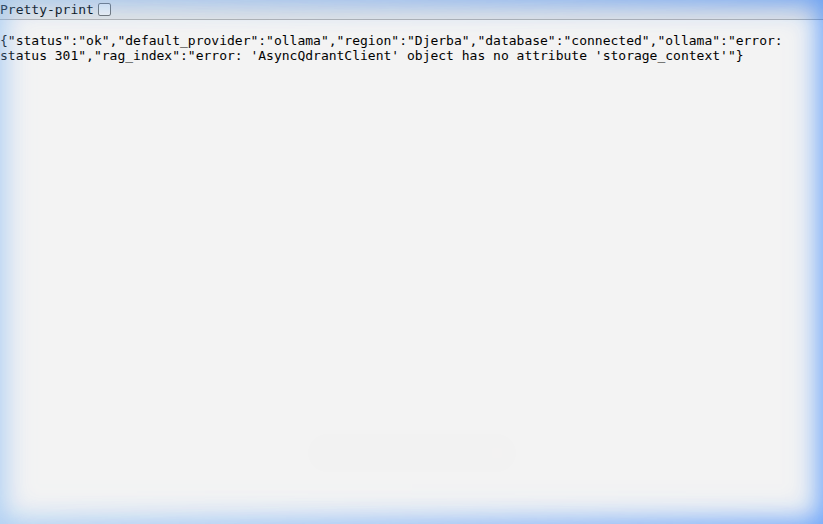
\includegraphics[width=0.7\textwidth]{diagrams/screen_06_health_endpoint.png}
    \caption{Réponse de l'endpoint GET /health}
    \label{fig:health_endpoint}
\end{figure}

\subsection{Tableau de Bord Administrateur}

Le tableau de bord administrateur comprend deux fonctionnalités principales~:

\textbf{Reconstruction manuelle de l'index RAG.} Bien que la réindexation incrémentale via les
écouteurs SQLAlchemy soit le mécanisme normal de mise à jour, un administrateur peut déclencher
une reconstruction complète via l'endpoint \texttt{POST /admin/rebuild-index}. Cette opération
est utile lors du premier déploiement, après une corruption détectée, ou lors de migrations de
schéma majeures.

\textbf{Consultation des métriques système.} L'endpoint \texttt{GET /metrics} (non documenté
dans l'API publique) expose des métriques Prometheus-compatibles~: nombre de requêtes par
endpoint, latence moyenne, taux d'erreur, taille de l'index RAG, nombre de bras LinUCB actifs.

\subsection{Documentation API OpenAPI}

FastAPI génère automatiquement une documentation interactive OpenAPI (Swagger UI) accessible via
l'endpoint \texttt{/docs}. La figure~\ref{fig:api_docs} montre la page de documentation avec
l'ensemble des 12 endpoints du système.

\begin{figure}[H]
    \centering
    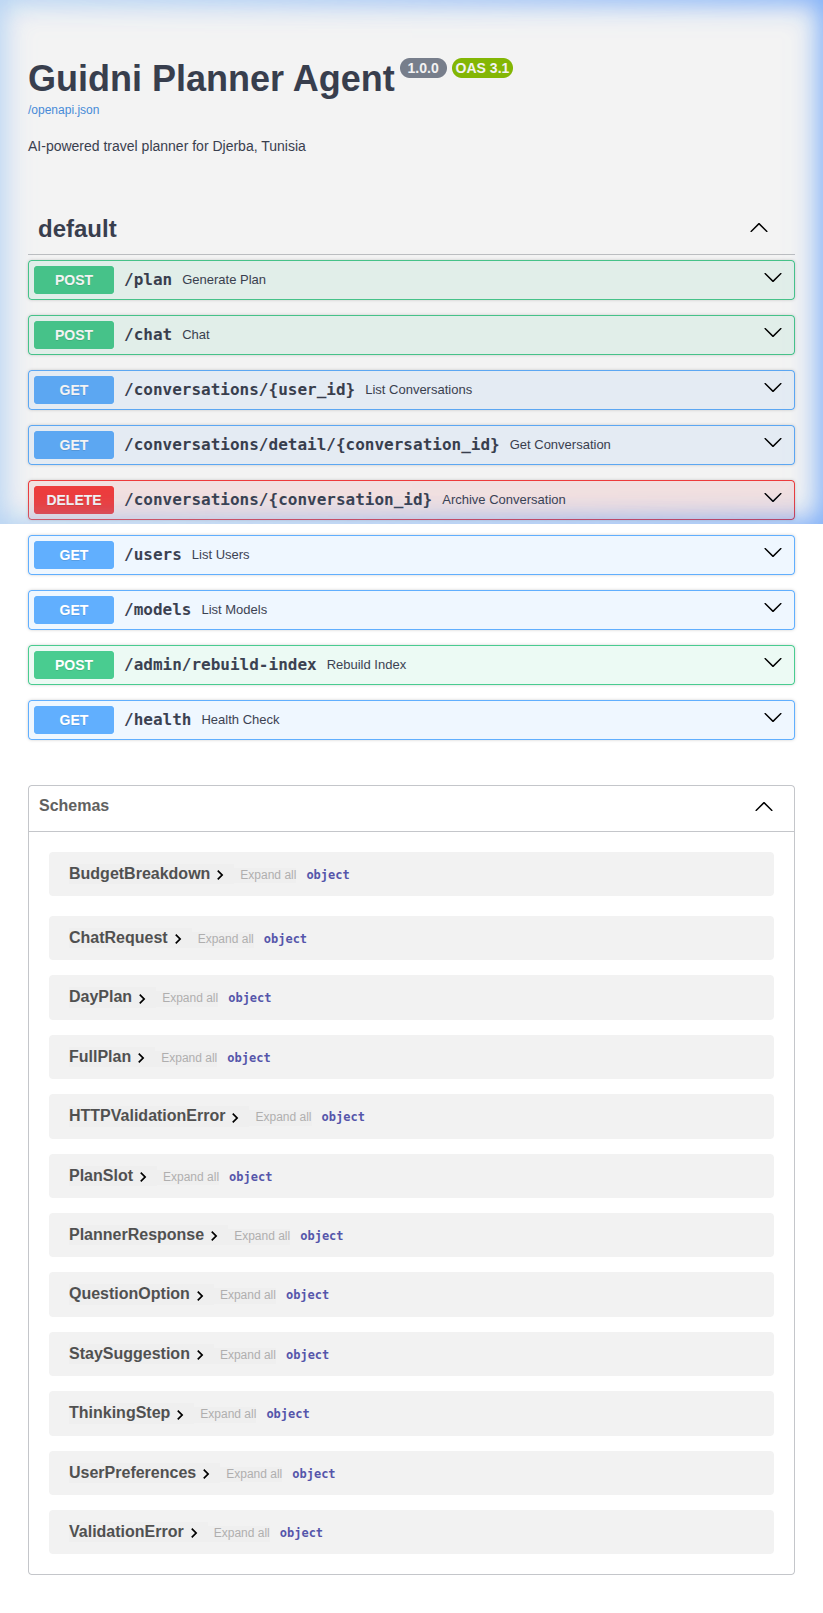
\includegraphics[width=0.85\textwidth]{diagrams/screen_A4_api_docs.png}
    \caption{Documentation API OpenAPI générée automatiquement}
    \label{fig:api_docs}
\end{figure}

Chaque endpoint inclut~:
\begin{itemize}
    \item La méthode HTTP et le chemin.
    \item La description de la fonctionnalité.
    \item Les schémas de requête (corps, paramètres, headers).
    \item Les schémas de réponse (succès et erreurs).
    \item Les codes d'erreur possibles (400, 404, 422, 500).
\end{itemize}

\subsection{Journalisation Rotative}

Le système de journalisation est configuré dans \texttt{main.py} avec deux handlers~:

\begin{lstlisting}[language=Python, caption={Configuration du logging rotatif}]
from logging.handlers import RotatingFileHandler
import logging

# Handler INFO (10 MB max, 5 backups)
info_handler = RotatingFileHandler(
    "logs/app_info.log", maxBytes=10*1024*1024, backupCount=5
)
info_handler.setLevel(logging.INFO)
info_handler.setFormatter(formatter)

# Handler DEBUG (50 MB max, 3 backups)
debug_handler = RotatingFileHandler(
    "logs/app_debug.log", maxBytes=50*1024*1024, backupCount=3
)
debug_handler.setLevel(logging.DEBUG)
debug_handler.setFormatter(formatter)

logger.addHandler(info_handler)
logger.addHandler(debug_handler)
\end{lstlisting}

Cette configuration garantit que les logs ne remplissent pas le disque tout en conservant un
historique suffisant pour le débogage post-mortem.

\subsection{Scénario de Démonstration Complète}

La démonstration finale couvre le scénario utilisateur suivant~:

\begin{enumerate}
    \item \textbf{Arrivée~:} Un touriste famille arrive sur la plateforme, souhaite planifier
          un séjour de 3 jours à Djerba avec un budget de 1500 TND.
    
    \item \textbf{Conversation~:} Il envoie un message en français~: \og{}Je veux un plan pour
          3 jours à Djerba en famille avec 2 enfants, budget 1500 TND.\fg{}
    
    \item \textbf{Planification~:} L'agent génère un plan structuré jour par jour avec activités,
          restaurants et hébergements, affiché dans l'interface chat (figure~\ref{fig:demo_plan}).
    
    \item \textbf{Modification~:} L'utilisateur demande~: \og{}Peux-tu remplacer l'activité du
          jour 2 par quelque chose de plus adapté aux enfants~? \fg{} L'agent régénère le jour 2.
    
    \item \textbf{Recommandations~:} En parallèle, la sidebar affiche des recommandations
          personnalisées qui s'adaptent aux clics de l'utilisateur.
    
    \item \textbf{Health Check~:} L'administrateur consulte \texttt{/health} qui retourne
          \texttt{"status": "healthy"}.
\end{enumerate}

\begin{figure}[H]
    \centering
    
\includegraphics[width=0.85\textwidth]{diagrams/screen_A4_chat_interface.png}
    \caption{Interface de chat avec plan généré (démonstration)}
    \label{fig:demo_plan}
\end{figure}

\begin{figure}[H]
    \centering
    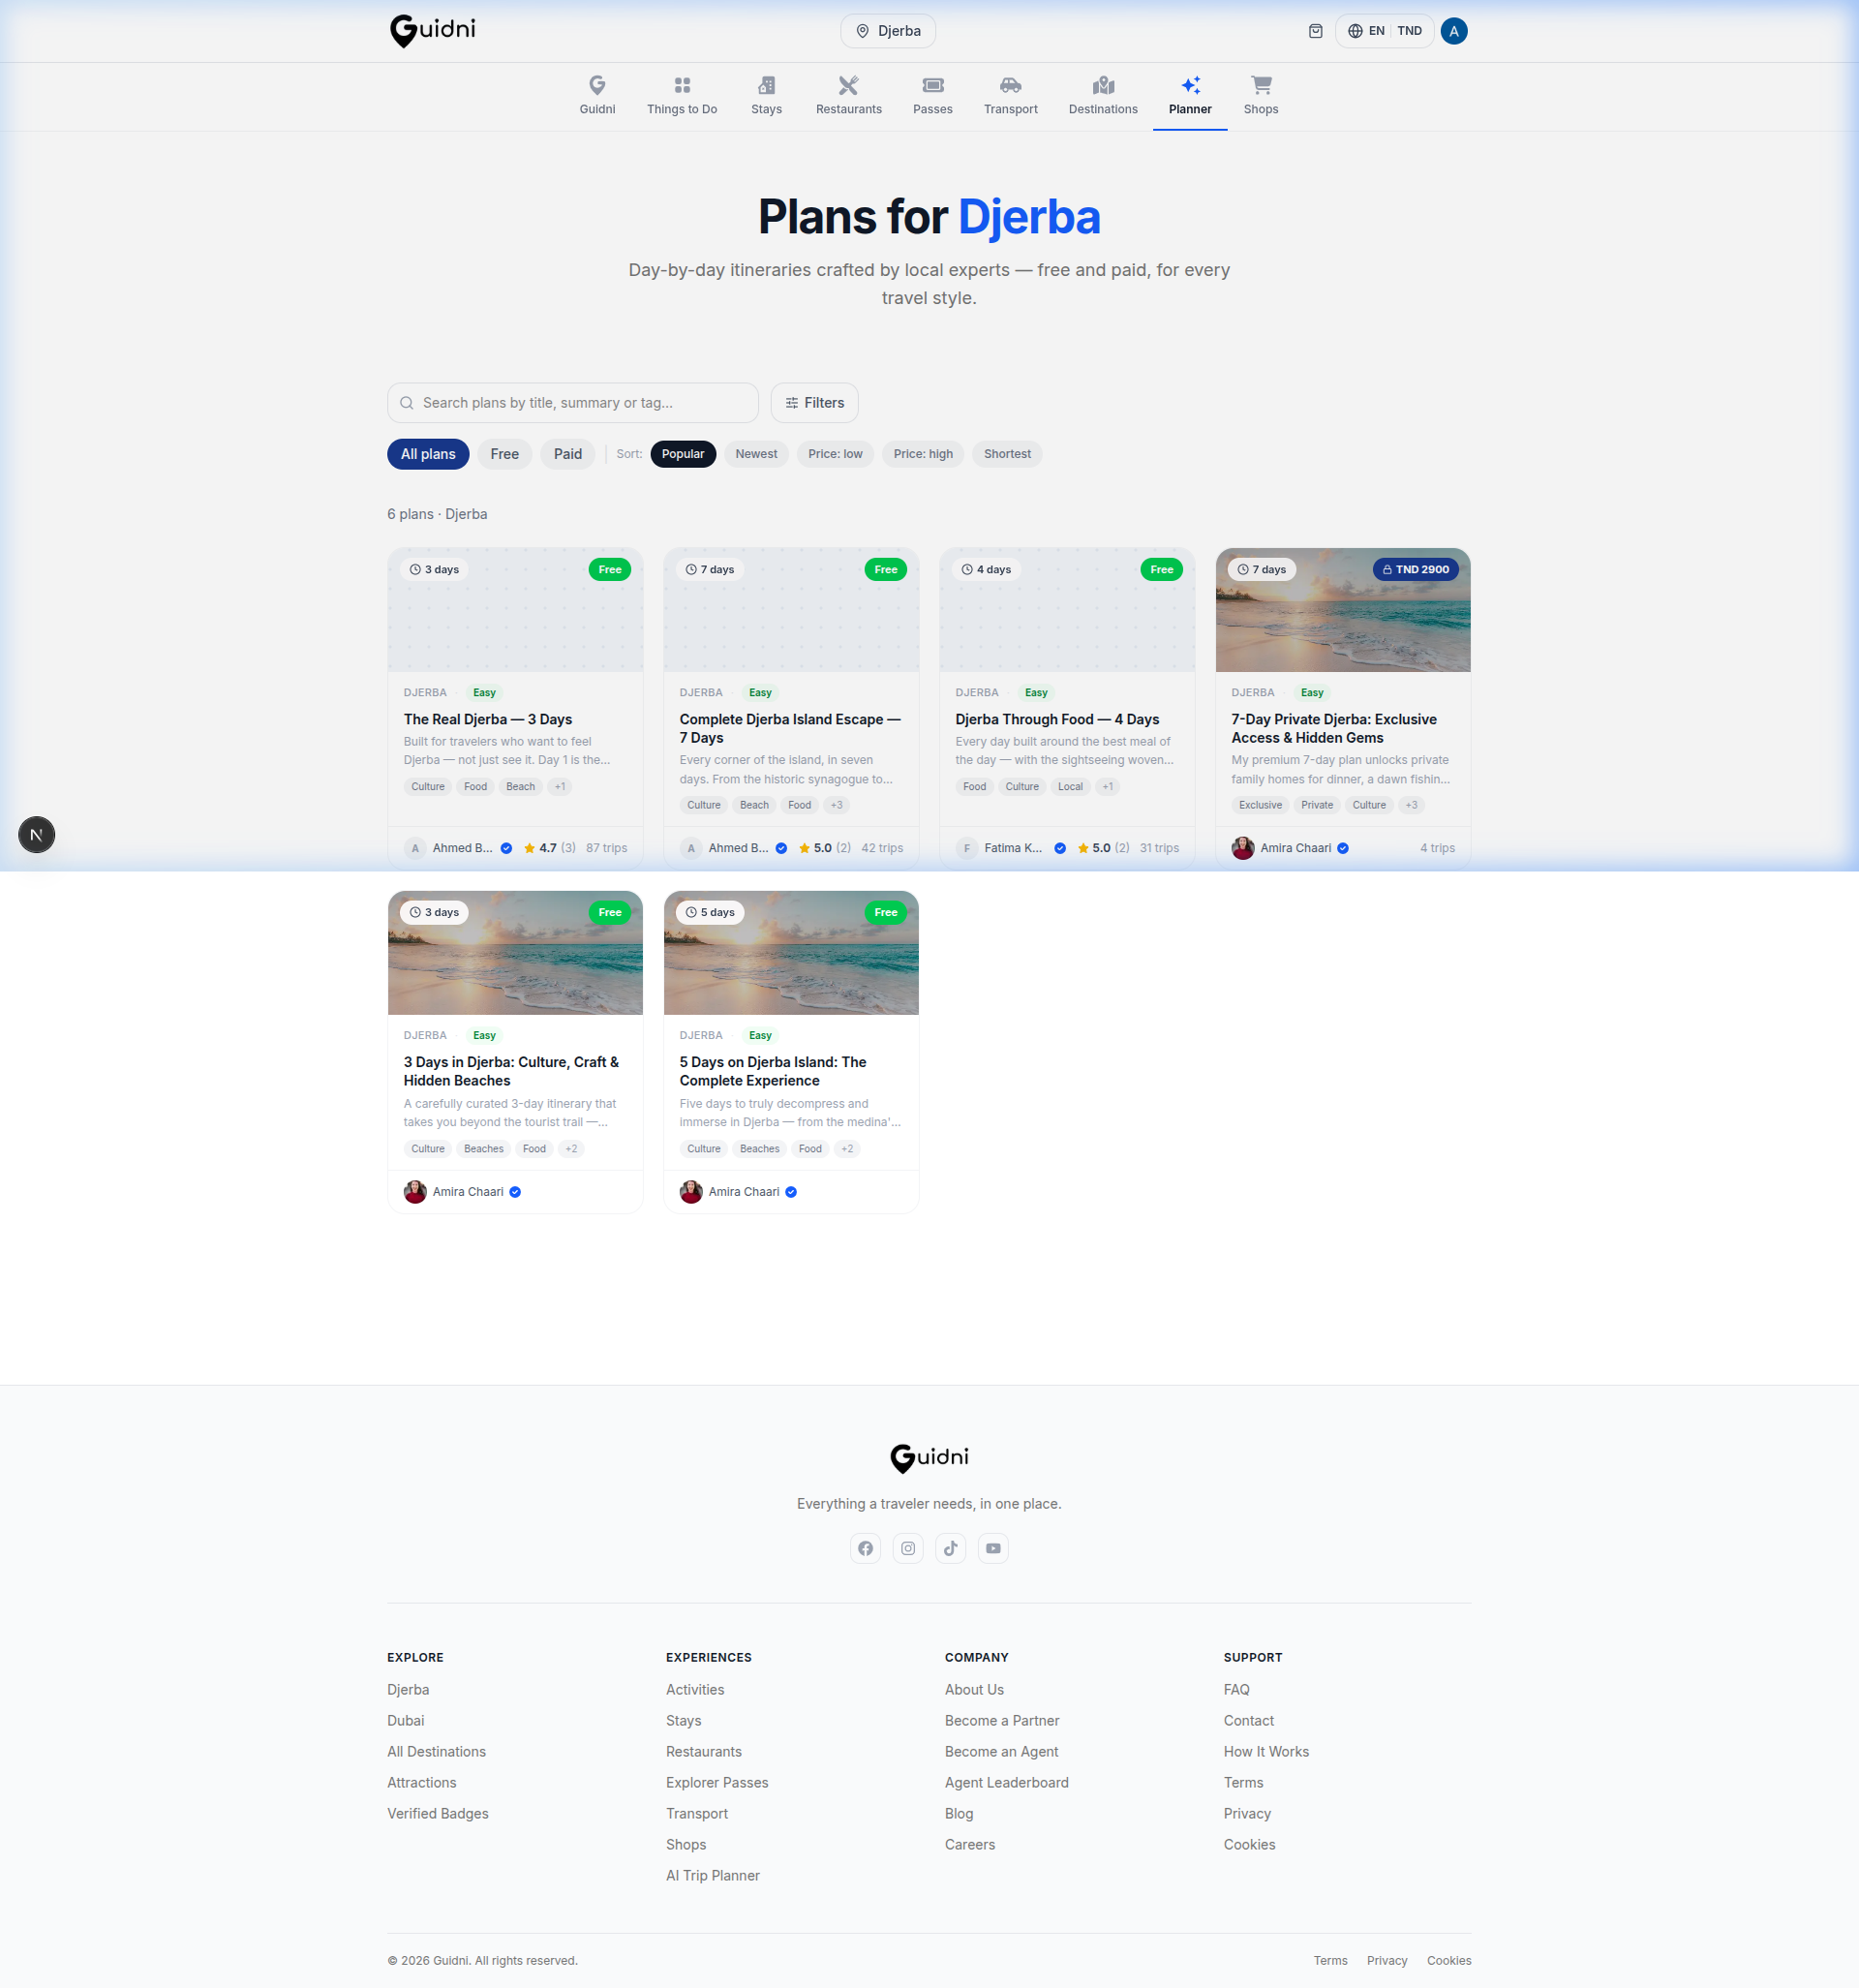
\includegraphics[width=0.85\textwidth]{diagrams/screen_A4_plan_output_full.png}
    \caption{Sortie complète du plan avec étapes de réflexion}
    \label{fig:demo_plan_full}
\end{figure}


% ────────────────────────────────────────────────────────────────
\section{Tests d'Intégration}
% ────────────────────────────────────────────────────────────────

Les tests d'intégration du sprint 4 vérifient la coexistence pacifique des deux sous-systèmes~:

\begin{table}[H]
    \centering
    \caption{Tests d'intégration — Sprint 4}
    \label{tab:integration_tests_s4}
    \small
    \begin{tabular}{p{4cm} p{5cm} p{3cm} p{3cm}}
        \toprule
        \textbf{Test} & \textbf{Description} & \textbf{Résultat attendu} & \textbf{Statut} \\
        \midrule
        IT-4.1 & Agent + Reco partagent DB PostgreSQL & Aucun conflit de lock, transactions isolées & Pass \\
        IT-4.2 & Réindexation RAG n'interrompt pas scoring LinUCB & Latence < 150 ms pendant rebuild & Pass \\
        IT-4.3 & Jobs nocturnes n'interfèrent pas avec requêtes chat & Pas de timeout, logs propres & Pass \\
        IT-4.4 & Health check retourne healthy en conditions normales & status=healthy, HTTP 200 & Pass \\
        IT-4.5 & Rebuild-index complet avec 500+ annonces & < 5 minutes, aucun échec embedding & Pass \\
        \bottomrule
    \end{tabular}
\end{table}


% ────────────────────────────────────────────────────────────────
\section{Conclusion du Sprint 4}
% ────────────────────────────────────────────────────────────────

Ce quatrième sprint a permis d'intégrer avec succès les deux sous-systèmes développés
indépendamment (agent planificateur et moteur de recommandation) dans une plateforme unifiée
opérationnelle. Les endpoints de santé fournissent une visibilité en temps réel sur l'état du
système, le tableau de bord administrateur permet les opérations de maintenance nécessaires, et
la documentation OpenAPI facilite l'adoption par les développeurs frontend.

Le sprint a été présenté lors d'une Sprint Review avec le superviseur académique, démontrant
le scénario utilisateur complet de bout en bout. Les feedbacks recueillis ont validé la
cohérence globale de la plateforme et la qualité de l'intégration.

Avec ce sprint, le cycle de développement Scrum est terminé. Les quatre sprints ont livré~:
\begin{itemize}
    \item \textbf{Sprint 1~:} Agent conversationnel LangGraph avec RAG multilingue.
    \item \textbf{Sprint 2~:} Moteur de recommandation LinUCB avec apprentissage en ligne.
    \item \textbf{Sprint 3~:} Tests complets et évaluation empirique des performances.
    \item \textbf{Sprint 4~:} Intégration, déploiement et démonstration finale.
\end{itemize}

Le chapitre suivant conclut le rapport en synthétisant les contributions majeures et en
proposant des pistes de travaux futurs.
